\section{Implantation d'éoliennes}

Les parties \ref{part:site_M} et \ref{part:site_F} sont indépendantes.

Après étude, les autorités d'une ile isolée ont décidé d'installer une éolienne pour répondre aux besoins énergétiques de leur communauté. L'éolienne choisie fonctionne lorsque le vent atteint au moins 8 n\oe uds et il faut l'arrêter lorsque le vent atteint ou dépasse les 48 n\oe uds. 

\subsection{\'Etude des vitesses du vent sur le site M}\label{part:site_M}

Les autorités décident de mesurer pendant un mois, à l'aide d'un anémomètre, la vitesse du vent sur le site M, au sommet d'une montagne. Une mesure est effectuée chaque jour.

Les résultats obtenus sont présentés dans la tableau de la figure \ref{tab:site_M} (le mois comporte 30 jours) :

\begin{figure}[h]
	\begin{center}
		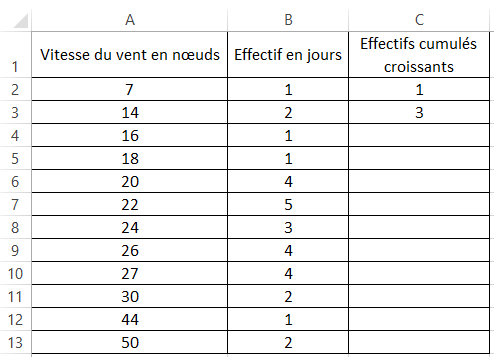
\includegraphics[scale=0.8]{eoliennes2}
	\end{center}
\caption{\'Etude de la vitesse du vent sur le site M}
\label{tab:site_M}
\end{figure}

On peut y lire que la vitesse de 22 n\oe uds a été mesurée 5 jours.

\begin{questions}
	\question
		\begin{parts}
			\part Compléter les tableau ci-dessus.
			
			\part Donner une formule à placer en \textbf{\texttt{C3}} permettant, par recopie vers le bas, de calculer les effectifs cumulés croissants des jours du mois étudié.
			
			\part Calculer le pourcentage des jours du mois étudié où l'éolienne ne produirait pas d'électricité. 
		\end{parts}
	
	
	\question Déterminer l'étendue, la médiane, les quartiles et l'écart interquartile de cette série statistique.
	
	\question On appelle premier décile (noté $D_1$) la plus petite valeur de la vitesse du vent, telle qu'au moins 10 \% des valeurs de la série sont inférieures ou égales à $D_1$. On appelle neuvième décile (noté $D_9$) la plus petite valeur, telle qu'au moins 90 \% des valeurs de la série lui sont inférieures ou égales.
	\begin{parts}
		\part Expliquer pourquoi $D_1$ = 14.
		\part Déterminer $D_9$.
	\end{parts} 
	
\end{questions}

\subsection{\'Etude des vitesses du vent sur le site F}\label{part:site_F}

Un emplacement sur une falaise, appelé site F, a également été retenu. Le même mois que le site M, on a mesuré les vitesses du vent sur le site F.

La série des mesures effectuée est dans le diagramme en boite de la figure \ref{fig:comparaison}. Les extrémités du diagramme correspondent aux premiers et neuvième déciles.

\begin{questions}
	
	\question Lire sur le graphique les quartiles de cette nouvelle série.
	
	\question Calculer l'écart interquartile.
\end{questions}

\begin{figure}[b]
	\begin{center}
		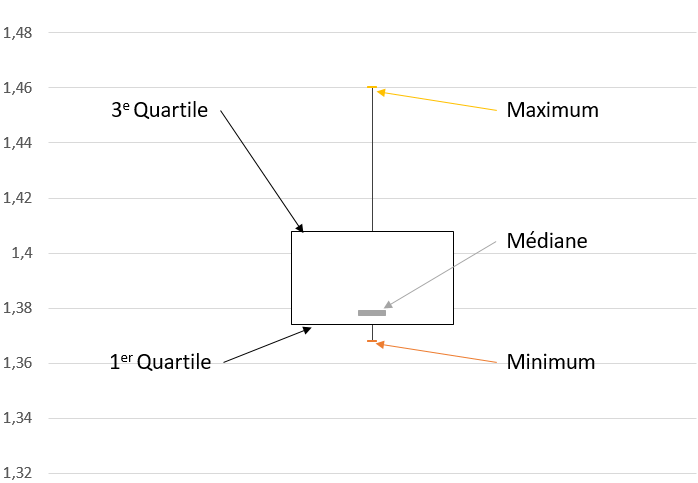
\includegraphics[scale=0.5]{../moustache}
	\end{center}
	\caption{Coparaison de la vitesse du vent sur les deux sites}
	\label{fig:comparaison}
\end{figure}

\subsection{Comparaison des sites}\label{part:comp}

\begin{questions}
	\question Représenter au-dessous du diagramme en boite fourni figure \ref{fig:comparaison}, celui de la série correspondant au site M. Prendre comme extrémités les premier et neuvième déciles.
	
	\question En comparant les diagrammes, sachant qu'une éolienne a un rendement optimal aux alentours de 23 n\oe uds, quel site paraît le plsu intéressant pour l'installation de l'éolienne ? Argumenter la réponse. 
\end{questions}